\documentclass[journal]{IEEEtran}
\ifCLASSOPTIONcompsoc
  % IEEE Computer Society needs nocompress option
  % requires cite.sty v4.0 or later (November 2003)
  \usepackage[nocompress]{cite}
\else
  % normal IEEE
  \usepackage{cite}
\fi


\usepackage{fixltx2e}
\usepackage{listings}

%JSON
\lstdefinelanguage{JSON}{
    basicstyle=\normalfont\ttfamily,
    showstringspaces=false,
    breaklines=true,
    frame=lines,
    morestring=[b]",
    morestring=[d]'
}

\lstdefinelanguage{hresource}{
    %language=html,
    basicstyle=\ttfamily,
    breaklines=true,
    moredelim=[s][\textbf]{rel="hresource}{"},
    moredelim=[s][\textbf]{class="}{"}
}


\usepackage{graphicx}

\begin{document}
%
% paper title
% can use linebreaks \\ within to get better formatting as desired
\title{MACHINE READABLE WEB SERVICE DESCRIPTIONS FOR AUTOMATED DISCOVERY AND COMPOSITION OF RESTFUL WEB SERVICES}

\author{\IEEEauthorblockN{
Dhananjay Balan\IEEEauthorrefmark{1},
Abil N George\IEEEauthorrefmark{1},
Akhil P M\IEEEauthorrefmark{1},
Deepak Krishanan\IEEEauthorrefmark{1},
and 
Dr. Abdul Nizar M \IEEEauthorrefmark{2}
}\\
\IEEEauthorblockA{\IEEEauthorrefmark{1} Department of Computer Science and Engineering, College of Engineering, Trivandrum}\\
\IEEEauthorblockA{\IEEEauthorrefmark{2}Professor, Department of Computer Science and Engineering, College of Engineering, Trivandrum}
}

% use for special paper notices
%\IEEEspecialpapernotice{(Invited Paper)}




% make the title area
\maketitle
`

\begin{abstract}
%\boldmath
Restful web services are getting popular today. Most of the service providers are moving to REST based services due to its simplicity and popularity. Even with this much adoption rate, creation of mashups is a himalayan task for an average web developer. Many solutions had been proposed for adding semantics to RESTful web services to automate discovery and composition of services. However they suffer from many problems like, biased towards SOAP based web services,need a separate file for machine parsable descriptions and more. The existing automated mahsup creation service faces scalability issues. The need of the hour is an highly scalable system to reduce as much human intervention as possible for the discovery and composition of the RESTful web services. In this paper, we proposed a microformat like grammar added to the existing service documentation to double them as machine readable. It also uses RDF descriptions at the backend in order to provide strong interlinking among resources, which the end users are not aware of.
\end{abstract}


\begin{IEEEkeywords}
Semantic Web, intelligent agents, web service, semantic web service, REST, RESTful architecture, service discovery, service composition, Microformats, Poshformats, RDF
\end{IEEEkeywords}

% For peer review papers, you can put extra information on the cover
% page as needed:
% \ifCLASSOPTIONpeerreview
% \begin{center} \bfseries EDICS Category: 3-BBND \end{center}
% \fi
%
% For peerreview papers, this IEEEtran command inserts a page break and
% creates the second title. It will be ignored for other modes.
\IEEEpeerreviewmaketitle



\section{Introduction}

REST defines a set of architectural principles for designing web services that uses a Resource Oriented approach compared to SOAP based services, which uses RPC semantics. REST is light-weight compared to SOAP which packs a lot of complexity with the implementation of SOAP envelopes and Header. SOAP messages are formatted in XML while we can use XML or JSON with RESTful services for sending and receiving data. 

REST provides a set of architectural constraints that, when applied as a whole, emphasizes scalability of component interactions, generality of interfaces, independent deployment of components, and intermediary components to reduce interaction latency, enforce security, and encapsulate legacy systems. REST uses Uniform Resource Indicators(URIs) to locate resources.Web developers are shifting to REST based services due to its simplicity and wide adoption rate as a standard for creating web services. Most of the companies now provides RESTful services like google,yahoo,amazon,facebook etc.

Mashups are formed by integrating  different services. They can combine data or functionality from two or more sources to create  new services. Early mashups were developed manually by enthusiastic programmers. More sophisticated approaches are in need as the use of mashuped services are increased in day to day life. This led to the thought of automating mashup creation so that machines can intelligently create mashups with minimal human intervention.

Earlier approaches of automated mashup creation sticks to the use of an external file for service description which only machine can understand. This gives additional overhead to developers for maintaining machine readable descriptions parallel to human readable documentations. The microformat \cite{kopecky2008hrests} like approach is simple and easy to use,hence provides low entry barriers for web developers. It uses existing service descriptions in HTML to double them as machine readable descriptions by adding annotations to it such that it is not visible in markups.

There exists so many mashup editors which can automate mashup creation like Yahoo pipes\cite{pip}, Google Mashup Editors(GME), Microsoft Popfly etc.Yahoo pipes is a free online service with a drag and drop interface to aggregate,manipulate and mashup content from around the web.You can create your own custom RSS feeds with Yahoo Pipe that pull in content from a variety of sources and filter it so that you only see the most relevant news stories.However Yahoo Pipes faces many drawbacks. It cannot create a mashup between any pair of services.Also Yahoo Pipes is not scalable since lack processing power. It fails to generate results while processing complex regex from far multiple locations, with hundreds of posts every minutes.

GME is the  mashup editor service from Google.Compared to Yahoo Pipes Google Mashup Editor wins in terms of power and flexibility. It allows to use coding in javascript,HTML,CSS etc along with the interactive interface. Microsoft Popfly is the simplest mashup editor which can be used as entry point for web developers. However both of these services were discontinued. 

\section{Related Works}
Many solutions had been proposed for formally describing RESTful web services. These proposals approach the problem  from different directions each providing a novel way of addressing the issue at hand. Most of these solutions were member submissions to the W3C but there is hardly any consensus on one global standard.

\subsection{Web Service Description Language (WSDL) 2.0}
WSDL 2.0\cite{chinnici2007web} is an extension of the Web Service Description Language (WSDL)that was used to describe traditional SOAP based services. WSDL 2.0 supports describing RESTful services by mapping the HTTP methods into explicit services available at the given URLs. So every resource will translate into 4 or fewer different services: GET, POST, PUT and DELETE. 
      
The advantage of WSDL 2.0 is that it provides a unified syntax for describing both SOAP based and RESTful services. It also has very expressive descriptions where you can define the specific data type, the cardinality and other advanced parameters for each input type. 
   
However, WSDL 2.0 requires RESTful services to be viewed and described from a different architectural platform: that of traditional RPC-like services. This forceful conversion negates many of the advantages of the RESTful philosophy. In addition, the expressiveness of the format comes at the price of losing the simplicity achieved by moving to the RESTful paradigm. These verbose files are not the easiest to be written by hand and also impose a maintenance headache. Hence, WSDL files are typically generated with the help of some tools. Further, WSDL descriptions are external files based on XML syntax that the developer has to create and maintain separately. 

\subsection{Web Application Description Language (WADL)}
Web Application Description Language (WADL)\cite{hadley2006web} is another XML based description language proposed by Sun Microsystems. Unlike WSDL, WADL is created specifically to address the description of web applications, which are usually RESTful services. WADL documents describe resources instead of services but maintain the expressive nature of WSDL. 
WADL still has some of the concerns associated with WSDL in that they still requires an external XML file to be created and maintained by the developer. It also results in boilerplate code. 

\subsection{hRESTS} 
hRESTS\cite{kopecky2008hrests} is a Microformat that attempts to fortify the already existing service documentations with semantic annotations in an effort to reuse them as formal resource descriptions. The Microformat uses special purpose class names in the HTML code to annotate different aspects of the associated services. It defines the annotations service, operation, address, method, input and output. A parser can examine the DOM tree of an hRESTS fortified web page to extract the information and produce a formal description. 

hRESTS is a format specifically designed for RESTful services and hence avoids a lot of unnecessary complexities associated with other solutions. It also reduces the efforts required from the developer since he no longer needs to  maintain a separate description of the service.   

One downside with hRESTS is that, despite being specifically designed for REST, it still adheres to an RPC-like service semantics. It is still required to explicitly mention the HTTP methods as the operations involved. Moreover, instead of representing the attributes of a resource, it attempts to represent them as input-output as in traditional services. This results in a lot of unnecessary markup.

\subsection{SA-REST}

Similar to hRESTS, SA-REST\cite{gomadam2010sa} is also a semantic annotation based technique. Unlike hRESTS, it uses the RDFa syntax to describe services, operations and associated properties. The biggest difference between them is that SA-REST has some built in support for semantic annotations whereas hRESTS provides nothing more than a label for the inputs and outputs. SA-REST uses the concept of lifting and lowering schema mappings to translate the data structures in the inputs and outputs to the data structure of an ontology, the grounding schema, to facilitate data integration. It shares much the same advantages and disadvantages as the hRESTS format. In addition, since SA- REST is strictly based on RDF concepts and notations, the developer needs to be well aware of the full spectrum of concepts in RDF.

\subsection{SEREDASj} 
SEREDASj\cite{lanthaler2011semantic}, a novel description method addresses the problem of resource description from a different perspective. While the other methods resort to the RPC-like semantics of input-operation-output, SEREDASj attempts to describe resources in their native format: as resources with attributes that could be created, retrieved, updated and deleted. This helps to reduce the inherent difference between operation oriented and resource oriented systems. The method also emphasizes on a simple approach that provides a low entry  barrier for developers.

One interesting aspect about SEREDASj is that it uses JSON (JavaScript Object Notation)[15] to describe resources. JSON is an easy and popular markup technique used on the web - especially with RESTful service developers. The advantage is that, the target audience is already familiar with the notation used for markup and can reduce friction when it comes to adoption.
         
SEREDASj, however, addresses the documentation and description in the reverse order. You can create the description in JSON first and then generate the documentation from this. This can increase upgrade effort required for existing services and is not very flexible. It is still possible to embed these JSON descriptions into existing documentation but it floats as a data island, separated from the rest of the HTML page. This, again, causes some duplication of data between the documentation and the description and causes a maintenance hurdle. 

\section{Service Description}
\label{sec:ServiceDescription}
Services are described using special purpose annotations in the HTML code. These annotations are specified in the class attribute of the associated tags. This attribute is usually used for classification of HTML elements and also as selectors for JavaScript access and to style elements via CSS. Using special purpose annotations as class names help us to reuse whatever is already provided by HTML and JavaScript. Following annotations are proposed for describing resources in a RESTful API.

\subsection{General Annotations}
\begin{enumerate}

\item {\bf hresource}: This is the root annotation that marks the resource description. All other annotations are contained within an element marked with {\it class="hresource"}. A client parsing a page could treat the presence of this annotation as an indication of the existence of a resource description on the page. Unless all other annotations are encapsulated in an hresource, they will not be parsed.

\item {\bf name} :Annotates the name of the resource. This can be any human readable name and need not have any programming significance.

\item {\bf url/uri}: Annotates the URL at which the resource is accessible.
\end{enumerate}

\subsection{Annotation Of Attributes}

\begin{enumerate}
\item {\bf attribute}: Annotates an attribute/property of the resource. All attributes of a resource should be annotated with this annotation. Specific characteristics of the attribute could be further specified by more annotations that are used together with the attribute annotation.

\item {\bf required}: Indicates a required attribute. This annotation is always used along with the attribute annotation.

\item {\bf queryable}:  Indicates an attribute that may be provided in the HTTP querystring during a GET operation to filter the results. This annotation is always used along with the attribute annotation.

\item {\bf read-only}:  Indicates a read-only attribute. A read-only attribute may be retrieved during a GET operation but may not be included in a POST or a PUT. This annotation is always used along with the attribute annotation.write-once: Indicates a write-once attribute that can be specified only during the create operation (POST) but not during update (PUT). This annotation is always used along with the attribute annotation.

\item {\bf guid}: Indicates if an attribute is a globally unique identifier for the resource that could be used across multiple services.
\item {\bf Comment}: Provides a human-readable description of the attribute. This should be descendant of parent of attribute node

\item {\bf hresource-datatype}: Annotates the datatype of the attribute.This should be descendant of parent of attribute node.For permissible types see table: \ref{tab:data_types}

\begin{table}
    \centering
    \begin{tabular}{|l|l|}
    \hline
    Data Type      & Description                    \\ \hline
    Integer or Int &  32 bit integer                \\ \hline
    float          & floating point number          \\ \hline
    Int64          &  64 bit integer.               \\ \hline
     Range         &  Boolean or Bool               \\ \hline
    Date or Time   & should specify date formatting \\ \hline
    Timestamp      & Timestamp of entity            \\ \hline
    \end{tabular}
    \caption{Data types}
    \label{tab:data_types}
\end{table}

{\bf eg}: Range(0.0,1.0) specifies floating point number between 0 and 1 and Range(0,1) specifies integer between 0 and 1.
\end{enumerate}



\subsection{Annotation of Methods}
Attribute can be input or output or both. Originally REST resource can be considers as bundle of attributes, each of which may have restriction on their access. But most of existing REST resources is specified as input/output of HTTP Methods ( GET,POST,PUT,DELETE).   

\begin{enumerate}
\item {\bf method}: This is the root annotation that marks the permissible method. It contains following sub-annotations
\begin{itemize}
\item {\it type}: HTTP request type. GET,POST,PUT,DELETE
\item {\it input}:  (optional) input attribute name
\item {\it output}: (optional) output attribute name
\item {\it header}: (optional) attributes that should be passed as header to HTTP request
\end{itemize}
\end{enumerate}

\subsection{Annotation of Errors}

\begin{enumerate}
\item {\bf hresource-error}: This is the root annotation that marks the errors.It should contain two sub-annotation for each error:
\begin{itemize}
\item {\it error-code}:Specify the error code.
\item {\it comment}: Description of error.
\end{itemize}
eg:
\begin{lstlisting}[language=html,breaklines=true]
<li class="hresource-error">
    <code class="error-code">201</code>:
    <span class="comment">test failed</span>
</li>
\end{lstlisting}
\end{enumerate}

\begin{figure}[!ht]
    \centering
    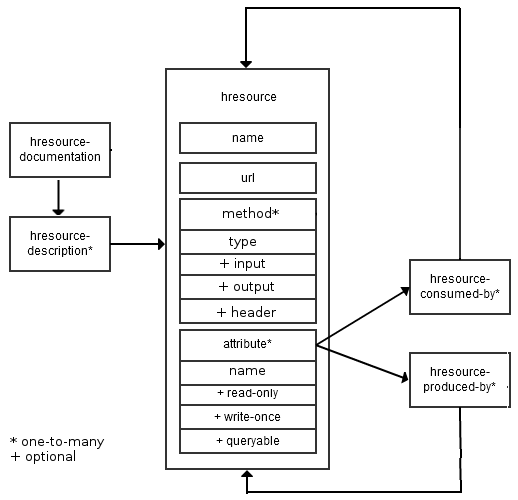
\includegraphics[width=3.5in]{images/rel_semantic.png}
    \caption{Relationship between the semantic annotations}
    \label{fig:rel_semantic}
\end{figure}

\subsection{Annotations For Linking Resources}
\begin{enumerate}
\item {\it Link to Super class}: When a resource is a subclass of another resource, this link is indicated by the rel attribute hresource-is-a. This implies that wherever the super class is accepted, the subclass is also accepted. For e.g., if a publisher defines a Book resource to provide a search of their catalog, they could annotate the resource to be a subclass of a more generic Book resource.

\begin{lstlisting}[language=html,breaklines=true]
<a rel="-is-a" href="http://dublincore.org/book/"> Book </a>
\end{lstlisting}

If there is another service from a bookshop that is known to accept a generic book resource for a purchase process, the client could infer that the specific book resource from the catalog would also be accepted there and use it.

For this linking to work properly, we need a core set of resources that can be extended by others. Fortunately, there is already a project named Dublin Core running that has defined many commonly used resources. We could reuse these resources for our purpose and use them as the root resources.

\item {\it Link to Consumers}: When an attribute of a service is consumed by another known service, this is annotated using \texttt{a rel attribute hresource-consumed-by}. This enables a software agent to find out what all can be done with the resource that it has already retrieved.

\begin{lstlisting}[language=html,breaklines=true]
<code class="attribute">ISBN</code>
Consumers:
<ul>
    <li rel="hresource-consumed-by">
    http://abc.com/buybook\#isbn
    </li>
    <li rel="hresource-consumed-by">
    http://xyz.com/rentbook\#isbn
    </li>
</ul>
\end{lstlisting}

\item {\it Link to Producers}: Similar to the link to consumers, services can annotate a link to a producer of one of its attributes. This helps reverse traversal of resources and also makes the system more peer-to-peer. This way, a link needs to be provided in either at one of the consumers or at the provider and an agent can identify this with link traversal. The annotation is made with the rel attribute \texttt{hresource-produced-by}.

The relationship between these semantic annotation is shown in figure \ref{fig:rel_semantic}.

\end{enumerate}


\section{Example REST{\it ful} web service}

%TODO
\vspace{50pt}
Consider a RESTful API with a ...

\textbf{\textit{TODO}}\\
\vspace{50pt}

The Listing.\ref{lst:Sample_HTML} depicts an annotation(according to Section.\ref{sec:ServiceDescription}[Service Description]) across an HTML description of above API. 

When above HTML page (Listing.\ref{lst:Sample_HTML}) is parsed,required information of API is generated as JSON,which is shown in  Listing.\ref{lst:Sample_JSON}.

Moreover we can also generate HTML documentary page from a JSON in specified format.

\lstinputlisting[language=hresource, frame=lines,
captionpos=b,caption=annotated HTML page, belowcaptionskip=4pt,
label=lst:Sample_HTML]{images/HTML.html}


\lstinputlisting[language=JSON,frame=lines
,captionpos=b,caption=JSON description generated from above HTML page, belowcaptionskip=4pt,
label=lst:Sample_JSON]{images/JSON.json}

\section{System implementation}

The proposed system currently addresses the composition of RESTful web services that represent resources using the JavaScript Object Notation (JSON). The system expects the services to return results to API queries as JSON objects and composes them as per the user specification. Extension of the same idea can enable the composition of XML based RESTful services. The system also includes an RDF conversion module that performs the automatic conversion process from Micro-format annotations to RDF\cite{rdf}.

The system uses a web UI at the client side for reading user input. The requests are handled by a server program developed in node.js that accepts requests from multiple client machines and handles them asynchronously. The server program acts as a proxy and is developed to enable the system to handle high volumes of client traffic. The server does the bulk of processing and also allows multiple cross domain HTTP calls with ease, which would otherwise be not possible with a client side implementation because of the same origin policy enforced by the modern web browsers.
The basic architecture of the system is as illustrated in \ref{fig:sys_arch}.
\begin{figure}[!ht]
    \centering
    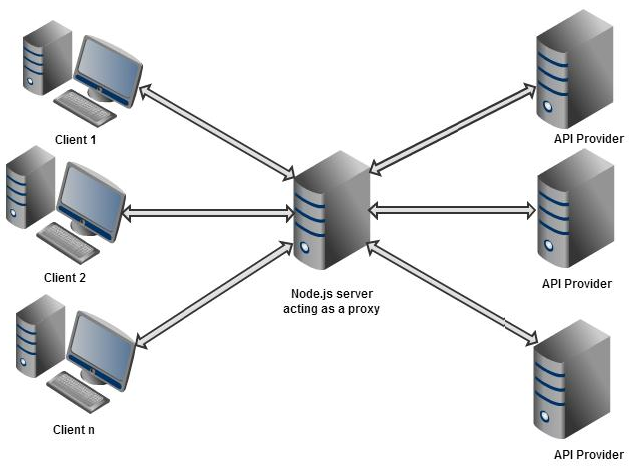
\includegraphics[width=3.5in]{images/sys_arch.png}
    \caption{System architecture}
    \label{fig:sys_arch}
\end{figure}

The system uses a parser module to parse the DOM tree of the annotated API Documentation page and extract the information embedded in it. Based on the information extracted from DOM tree, the web UI presented to the user is populated with a set of API operations that the system identifies and that can be composed. A workbench is presented to the user and a drag-drop based user interface enables the him/her to graphically describe the required composition of web services. Once the graphical design of the mash-up is complete and user submits it, information from the design is converted into an abstract internal representation that is passed to the server. The server now invokes the required API calls asynchronously and composes them as required and produces an HTML formatted output which is the required mash-up. The HTML output is then served back to the client system for the user.

The interaction flow in the system is illustrated in \ref{fig:interaction_flow}.
\begin{figure*}[!ht]
   \centering
    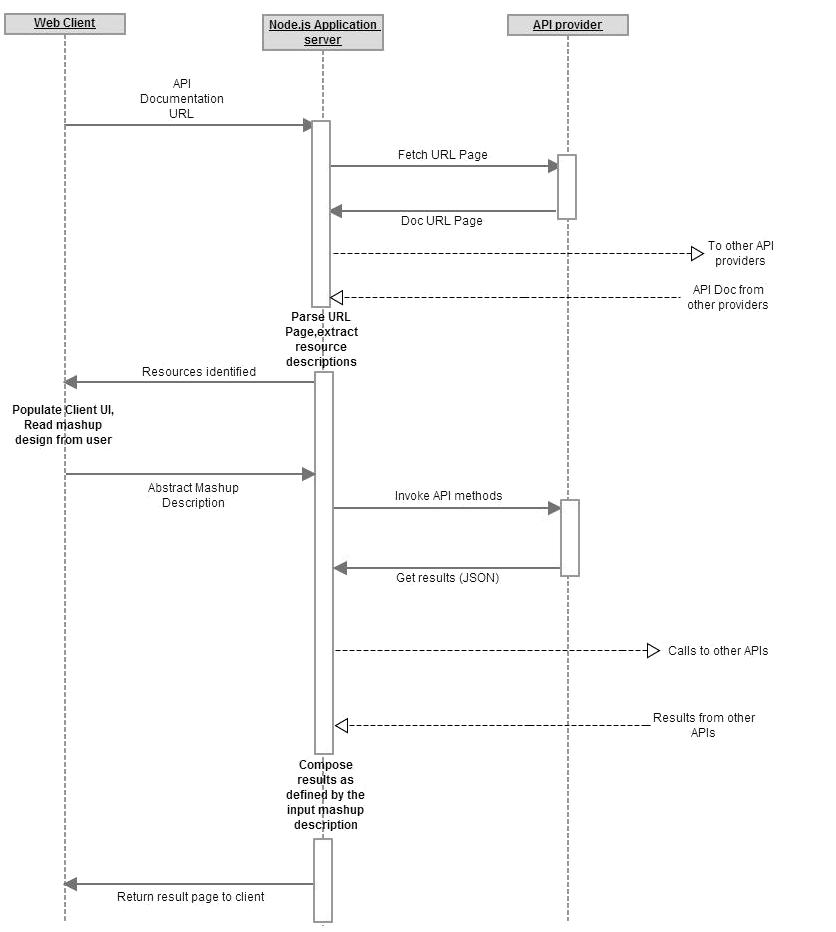
\includegraphics[width=6in] {images/seq.png}
    \caption{Interaction flow sequence}
    \label{fig:interaction_flow}
\end{figure*}


\subsection{Server Side Implementation}
\begin{figure}[!ht]
    \centering
    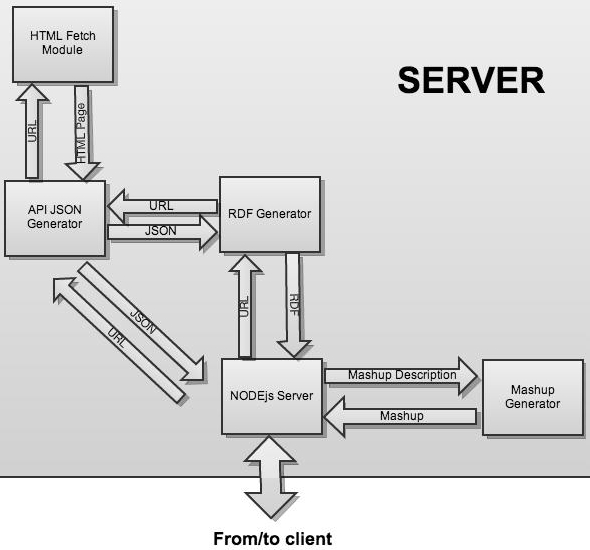
\includegraphics[width=3.5in]{images/server_arch.png}
    \caption{Server Architecture}
   \label{fig:server_arch}
\end{figure}
The architecture of the server is as illustrated in \ref{fig:server_arch}.Server primarily deals with providing three services:
\begin{enumerate}
    \item {\it Parsing API Documentation HTML}: Client side provides the URL of an annotated API     Documentation HTML page. The server fetches the required documentation page and passes 	the HTML DOM to the parser module (hrestsparser). The parser generates a JSON 	description of the annotated resources which is then passed to the client to populate the 	client UI. The parser uses XPath for the traversal of the DOM tree and hence platform 	neutral.
	\item {\it RDF Generation}: Client passes a URL to the server. The page is fetched by the RDF 	generator module. The page is parsed by the hRESTS parser module  to produce the output 	JSON. The produced-by,consumed-by,is-a relations in the annotated page forms a graph of 	resources each of which is required for the generation of the RDF description. The RDF 	generator module recursively traverses the graph and fetches each of the 	required resources 	up to some arbitrary level of nesting.
	\item {\it Request handling and mash-up generation}: The user specifies the required composition of 	services graphically in the client workbench. An abstract description of the required mash-up 	is generated at the client and is passed to the server as a JSON object. The server makes the 	required API invocations to fetch each of the resources to be composed into the final 	mash-up. The description JSON is parsed and the result resources are composed as specified 	producing an HTML output which is then served to the client system.
\end{enumerate}

\subsection{Client Side Implementation}
Client provides a simple drag and drop based user interface for mash-up design which can be implemented using jsPlumb\cite{jsplumb}. The elements in the UI are populated from the contents of the API documentations passed to the server. The different API calls can be simply dragged and dropped to the workbench and the inputs and outputs can be piped to one another by graphical connectors.

Client uses basic data structures which are simple JSON objects to keep track of attribute value or mapping .This forms a logical graph of the way in which the different service calls are composed. An abstract representation of the mash-up is created by traversing the graph. The traversal can be done by using a modified Depth First Search technique. The abstract representation is a JSON object which represents the initiation sequence for the API calls. This is then passed to the server.


\section{Conclusion and Future work}


Web is increasingly getting complex these days. Thousands of services spawn millions of requests each day. This work envisioned a intelligent web framework in which a service can create interconnections between different services compatible. It opens up a multitude of possibilities, including a higher layer manipulation of information for what it represents than how it is represented.

Popularization of services like ifttt\cite{ift} have given us the proof that this service is inevitable in the future of web, and if machines were able to parse the information constituted by entire internet it can do wonders that no one envisioned, so it can only be compared with magic.

The prototype mash-up editor created can intelligently mash the services based on annotations But it is also limited in some aspects. But we hope this direction deserves more exploration since it is relatively easy for the developer and the machine to follow. The prototype was implemented in different paradigms to verify the computational comparability.
The immediate future directions we would like to purse this works are
\begin{itemize}
\item Change to accommodate today's REST APIs. Most of the rest apis in use today does to conform to the RESTful paradigm. They use GET heavily to get most of the things done for performance purposes.
\item A tool to convert existing REST APIs. But this comes with lot of challenge. The above one for a start, adoption is another problem.
\end{itemize}

% use section* for acknowledgement
%\section*{Acknowledgment}
%The authors would like to thank...


% references section
\bibliographystyle{plain}
\bibliography{references}

% that's all folks
\end{document}


